\documentclass[pdftex, unicode, a4paper,12pt,oneside,utf8x, usehyperref]{report-gost}
\usepackage[pdftex]{graphicx}
\usepackage{wrapfig}
% \usepackage{floatflt}

\begin{document}
\title{Руководство по использованию программы SimplexSolver}
\author{Roman Tsisyk}
\thispagestyle{empty}
\begin{center}
\vspace{8cm}
\end{center}

\begin{figure}[ht]
\centering
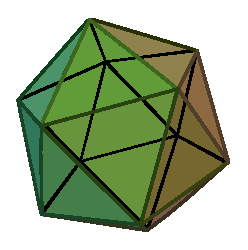
\includegraphics[width=0.8\textwidth]{img/simplex}
\end{figure}

\begin{center}
\LARGE{Simplex Solver} \\
\vspace{1cm}

\end{center}

\vspace{4cm}

\begin{center}
Руководство пользователя\\
\end{center}

\vspace{\fill}

\begin{center}
\Large{г. Барнаул, 2009}
\end{center}

\clearpage
\newpage
\thispagestyle{empty}
\begin{center}
\ \vspace\fill
\end{center}


© 2009, Роман Цисык <\href{mailto:roman@tsisyk.com}{roman@tsisyk.com}>.

Версия документа 1.0 от 25 мая 2009 г. для SimpleSolver версии 1.0.

SimplexSolver представляет собой свободное программное обеспечение.
Вы можете свободно распространять и/или изменять программу при соблюдении условий лицензии \href{http://www.gnu.org/licenses/gpl.html}{GNU General Public License}
(версии 3 или более поздней), опубликованной
\href{http://www.fsf.org/}{Фондом свободного программного обеспечения.}
Данная программа распространяется в надежде, что она будет полезной,
но без всякой гарантии, в том числе без связанной гарантии товарной пригодности
или пригодности для частного использования.

Данная документация и логотип программы распространяется на условиях лицензии \href{http://www.creativecommons.org/licenses/by-sa/3.0/}{Creative Commons Attribution ShareAlike 3.0}.
Вы можете без ограничений распространять их, изменять и использовать в любых (в том числе коммерческих) целях при условии указания оригинального авторства и сохранения данной лицензии в производных работах.

\newpage

\frontmatter % выключает нумерацию

\tableofcontents

\mainmatter %% включает нумерацию

\chapter{Общая информация}
SimplexSolver решает задачу линейного программирования (ЗЛП).
Задача линейного программирования заключается в нахождении
максимума или минимума линейной целевой функции при заданной системе линейных ограничений.

Основная задача линейного программирования может быть записана в следующем виде:
\begin{equation}
F(\vec{X}) = c_1 x_1 + c_2 x_2 + \hdots + c_n x_n \to max
\end{equation}
\begin{equation}
\label{limits}
\begin{cases}
\begin{matrix}
a_{11} x_1 & + & a_{12} x_2 & + & \hdots &a_{1n} x_n &\le & b_1 \\
a_{21} x_1 & + & a_{22} x_2 & + & \hdots &a_{2n} x_n &\le & b_2 \\
\vdots     & ~ & \vdots     & ~ & \ddots &\vdots     & \vdots & \vdots \\
a_{m1} x_1 & + & a_{m2} x_2 & + & \hdots &a_{mn} x_n &\le & b_m \\
\end{matrix} \\
\end{cases}
\end{equation}

Знаки неравенств \eqref{limits} могут быть как $\le$ и $\ge$, так и $=$.
В последнем случае говорят, что задача представлена в каноническом виде.

Поскольку отрицательные значения $x_{m}$ как правило не имеют экономического смысла,
то к системе ограничений \eqref{limits} часто добавляют условие $x_m \ge 0$. Программа предназначена в первую очередь для учащихся экономических специальностей, поэтому имеет естественное ограничение на не отрицательность искомых переменных.

Нецелые значения $x_{ij}$ иногда также не имеют экономического смысла. Допустим, эти переменные могут показывать количество единиц выпускаемой продукции и дробное значение не уместно в данном случае. Тогда к системе ограничений \eqref{limits} добавляют также условие целочисленности переменных. В этом случае говорят, что это задача целочисленного линейного программирования. Данная возможность предусмотрена в программе.

Обычно условия ЗЛП записывают в виде вектор-строки $\vec{С}$ коэффициентов при целевой функции, матрицы коэффициентов в системе ограничений \eqref{limits} и вектора $\vec{B}$ свободных членов этой системы.
\chapter{Алгоритм работы программы}
\section{Выделение начального базиса}
Для решения ЗЛП исходную матрицу ограничений необходимо представить в каноническом виде и выделить в ней начальный базис. Программа пытается найти базисные вектора в исходной системе уравнений, а при отсутствии таковых, добавляет в систему ограничений балансовые и искусственные переменные (используется метод искусственного базиса).
Данные переменные представляют собой разницу между запасами ресурсов и их потреблением. Коэффициенты при искусственных переменных в исходной функции обозначаются буквой $W$. Подразумевается, что $W$ бесконечно большое число, которое не повлияет на ход нахождения минимума функции.

Алгоритм программы сводит любую задачу к нахождению минимума. Для этого, при максимизации, коэффициенты при целевой функции умножаются на $-1$, что позволяет заменить задачу максимизации минимизацией.

\section{Нахождение оптимального опорного плана}
После выделения начального плана, программа начинает перемещение по вершинам симплекса в поисках оптимального опорного плана. Для этого составляются промежуточные симплекс-таблицы.

В столбцах $P_i$ строки $m+1$ находятся объективно-обусловленные оценки (решение двойственной задачи). Экономическая интерпретация данных оценок может быть различна, но как правило, данные оценки показывают степень важности каждого из ресурсов. В $m+2$ строке находится искусственная часть двойственных оценок, которая при успешном решении задачи обращается в ноль (это может означать, что все искусственные переменные исключены).

Вводимая в базис переменная определяется по максимальному неотрицательному значению в $m+2$ строке. В случае обращения всех значений в не искусственных столбцах $P_i$ строки $m+2$ в ноль, выполняется поиск максимального значения в $m+1$ строке. В случае отсутствия положительных неискусственных элементов в $m+2$ строке и равенству нулю значения в столбце $B$, выполняется поиск максимального элемента в $m+1$ строке над нулевыми элементами $m+2$. Следует учитывать, что искусственная переменная в базис вводится только один раз.

Выводимая из базиса переменная определяется по минимальному положительному элементу в столбце  $\theta$. Отсутствие в столбце положительных значений может говорить о невозможности нахождения оптимального плана. Компонент, находящийся на пересечении выбранного столбца и выбранной строки, называется направляющим.

После нахождения направляющего компонента и смены опорного плана (базиса), поиск решения продолжается вновь, вплоть до нахождения оптимального плана. Критерием остановки может служить отсутствие положительных элементов в $m+1$ строке.

В столбце $B$ $m+1$ строки находится текущее значение целевой функции, которое вычисляется как произведение управляющих переменных в базисе на коэффициенты функции. Сумма произведений искусственных переменных в базисе на $С_j = W$ сохраняется в $m+2$ строке.

\section{Нахождение целочисленного решения}

После нахождения оптимального опорного плана (то есть и решения задачи), программа проверяет условие целочисленности выбранных переменных. В случае, если одна из указанных переменных, не является целочисленной, то программа выполняется отсечение Гомори и смену базиса, после чего поиск оптимального целочисленного решения продолжается вновь.

\section{Вычисление интервалов устойчивости двойственных оценок}
Программа также умеет вычислять интервалы значений $\vec{С}$ и $\vec{B}$, в которых двойственные оценки сохраняют свое значение.

Для нахождения интервалов устойчивости свободных членов $B_m$, из симплекс-таблицы находится обратная матрица (она содержится в столбцах исходного опорного плана канонической задачи) и умножается на приращение вектора $\Delta b_i$. Все элементы решения должны быть неотрицательны, иначе решение будет недопустимым, т.е. базисное решение остаётся оптимальным до тех пор, пока оно допустимое. Для каждого ограничения находится интервал устойчивости, при котором двойственные оценки сохраняют свое значение.

Интервалы устойчивости коэффициентов целевой функции $С_m$ определяются исходя из величины двойственных оценок.
\chapter{Установка программы}
Программа поддерживает все основные платформы, в том числе Windows, Unix/X11 и MacOS. Для графического интерфейса используется библиотека Qt 4.5, поэтому данная библиотека должна быть установлена в системе.

\section{Особенности установки под платформу Windows}
Для установки программы следует использовать программу установки SimplexSolver-1.0-setup.exe, находящуюся в дистрибутиве программы и далее следовать инструкция мастера установки.

При установке будет предложено установить также необходимую версию библиотеки Qt, которая включена в дистрибутив программы и данный файл документации.

\section{Сборка из исходных текстов}
Вместе с дистрибутивом программы предоставляются исходные тексты, из которых программа может быть скомпилирована под любую другую платформу, в том числе Linux, Mac OS X, OpenSolaris или FreeBSD.

Для сборки программы необходимо сгенерировать Makefile. Для этого следует использовать команду qmake (входит в состав Qt). После генерации Makefile, программу можно скомпилировать, используя команду gmake (или nmake, зависит от платформы).

Вы можете использовать тексты программы в своих разработках при соблюдении лицензионного соглашения программы.


\chapter{Использование программы}
Главное окно программы состоит из двух вкладок: “Условия” и “Решение”.
В первой вкладке осуществляется ввод условий задачи. Во второй вкладке отображается ход решение и результат.
Внешний вид и оформление программы могут отличаться в зависимости от платформы, на которой будет запущена программа.

\begin{figure}[ht]
\centering
\includegraphics[width=\textwidth]{img/mainwindow.png}
\caption{Главное окно программы}
\end{figure}
\clearpage

\section{Ввод задачи}
Во вкладке “Условия” в первой строке необходимо задать целевую функцию (вектор-строка $\vec{C}$ и тип оптимизации.
Во всех остальных строках, кроме последней, наобходимо задать коэффициенты матрицы, знаки неравенств и значение свободных членов системы ограничений. В последней строке задаются ограничения целочисленности каждой из переменных.

Для добавления переменных и ограничений можно воспользоваться кнопками cнизу таблицы или контекстным меню (на правую клавишу мыши).
\begin{figure}[ht]
\centering
\includegraphics[scale=1.0]{img/contextmenu.png}
\caption{Контекстное меню таблицы}
\end{figure}

Пример. Задача задана в следующем виде:
\begin{equation}
 	F(\vec{X}) = x_1+x_2 \to max,
\end{equation}
\begin{equation}
\begin{cases}
x_1 + 5x_2 \le 10\\
7x_1 + 8x_2 \le 4\\
x_i \ge 0.
\end{cases}
\end{equation}
\clearpage
В окне программы это будет выглядеть следующим образом:
\begin{figure}[ht]
\centering
\includegraphics[scale=1.0]{img/problem1.png}
\caption{Задание условий задачи в программе}
\end{figure}

\section{Получение решения}
Во вкладке “Решение” отображается ход решения. В начале документа показана задача, приведенная к каноническому виду.

\begin{figure}[ht]
\centering
\includegraphics[scale=1.0]{img/canonical.png}
\caption{Задача в каноническом виде}
\end{figure}

Далее идут промежуточные симплекс-таблицы, которые могут быть полезны для понимания механизма работы алгоритма или более детального исследования задачи. Следует учитывать, что при нахождении максимума, оценки в $m+1$ и $m+2$ строках таблицы записаны с противоположными знаками. При отсутствии искусcтвенных переменных, $m+2$ строка не отображается.

\begin{figure}[hb]
\centering
\includegraphics[scale=1.0]{img/simplextable.png}
\caption{Симплекс-таблица}
\end{figure}
После таблиц отображается оптимальное значение функции $F(\vec{X})$ и значения соотвествующих переменных $x_{i}$ ввиде компонентов вектора $\vec{X}$.

\newpage
\clearpage

\begin{figure}[ht]
\centering
\includegraphics[scale=1.0]{img/result.png}
\caption{Результат}
\end{figure}

В самом конце указаны интервалы устойчивости $\vec{С}$ и $\vec{B}$, при которых двойственные оценки сохраняют свое значение.
\begin{figure}[hb]
\centering
\includegraphics[scale=1.0]{img/stability.png}
\caption{Интервалы устойчивости}
\end{figure}

\section{Сохранение результата}
Вывод программы можно сохранить в файл. В данной версии поддерживается формат OpenDocument Text (.odt), который в свою очередь может быть открыт популярным офисным пакетом OpenOffice.org, и формат HTML 4 (.html), который может быть просмотрен любым совместимым веб-браузером. Предусмотрена возможность отправки вывода программы на печать.


\chapter{Примеры решения задач}
\section{Пример I}

\renewcommand{\labelenumi}{\arabic{enumi})}
Задана ЗЛП с целевой функцией:
\begin{equation}
	F(\vec{X}) = x_1+x_2 \to max.
\end{equation}

Система ограничений имеет следующий вид:
\begin{equation}
\begin{cases}
20x_1+10x_2 \le 45\\
2x_1+7x_2 \le 14\\
x_i \ge 0 \\
\end{cases}
\end{equation}.

\subsection{Решение исходной ЗЛП}
Введем балансовые переменные и приведем к каноническому виду.
Для нахождения максимума, умножим целевую функцию на -1.

$$-F(\vec{X}) = -(-x_1-x_2) \to max$$
\begin{equation}
\begin{cases}
20x_1+10x_2+x_3=45\\
2x_1+7x_2+x_4=14\\
x_i, s_i \ge 0 \\
\end{cases}
\end{equation}

Составим таблицу и решим задачу симплекс-методом.

\begin{center}
\begin{tabular*}{\textwidth}{@{\extracolsep{\fill}}|c|c|c|c|c|c|c|c|c|}
\hline
$i$ & Базис & $C_i$ & B & $C_1 = -1$ & $C_2 = -1$ & $C_3 = 0$ & $C_4 = 0$ & $\Theta_i$ \\
\hline
$1$ & $P_3$ & $0$ & $45$ & $20$ & $10$ & $1$ & $0$ & $2,25$\\
$2$ & $P_4$ & $0$ & $14$ & $2$ & $7$ & $0$ & $1$ & $7$\\
\hline
$m+1$ & ~ & ~ & $0$ & $1$ & $1$ & $0$ & $0$ & ~ \\
\hline
\end{tabular*}
\end{center}
\begin{center}
\begin{tabular*}{\textwidth}{@{\extracolsep{\fill}}|c|c|c|c|c|c|c|c|c|}
\hline
$i$ & Базис & $C_i$ & B & $C_1 = -1$ & $C_2 = -1$ & $C_3 = 0$ & $C_4 = 0$ & $\Theta_i$ \\
\hline
$1$ & $P_1$ & $-1$ & $2,25$ & $1$ & $0,5$ & $0,05$ & $0$ & $4,5$\\
$2$ & $P_4$ & $0$ & $9,5$ & $0$ & $6$ & $-0,1$ & $1$ & $1,583$\\
\hline
$m+1$ & ~ & ~ & $-2,25$ & $0$ & $0,5$ & $-0,05$ & $0$ & ~ \\
\hline
\end{tabular*}
\end{center}
\begin{center}
\begin{tabular*}{\textwidth}{@{\extracolsep{\fill}}|c|c|c|c|c|c|c|c|c|}
\hline
$i$ & Базис & $C_i$ & B & $C_1 = -1$ & $C_2 = -1$ & $C_3 = 0$ & $C_4 = 0$ & $\Theta_i$ \\
\hline
$1$ & $P_1$ & $-1$ & $1,458$ & $1$ & $0$ & $0,05833$ & $-0,08333$ & $4,5$\\
$2$ & $P_2$ & $-1$ & $1,583$ & $0$ & $1$ & $-0,01667$ & $0,1667$ & $1,583$\\
\hline
$m+1$ & ~ & ~ & $-3,042$ & $0$ & $0$ & $-0,04167$ & $-0,08333$ & ~ \\
$m+1$ & ~ & ~ & $3,042$ & $0$ & $0$ & $0,04167$ & $0,08333$ & ~ \\
\hline
\end{tabular*}
\end{center}
Получен оптимальный план: $X^{опт} = (1,458;1,583)$, и оптимальное значение целевой функции $F^{опт} = 3,04$.

Тогда оптимальный план и значение двойственной симметричной ЗЛП:
\begin{align*}
	Y^{опт} = (0,042; 0,083),&~ Z^{опт} = 3,04.
\end{align*}

\begin{figure}[ht]
\centering
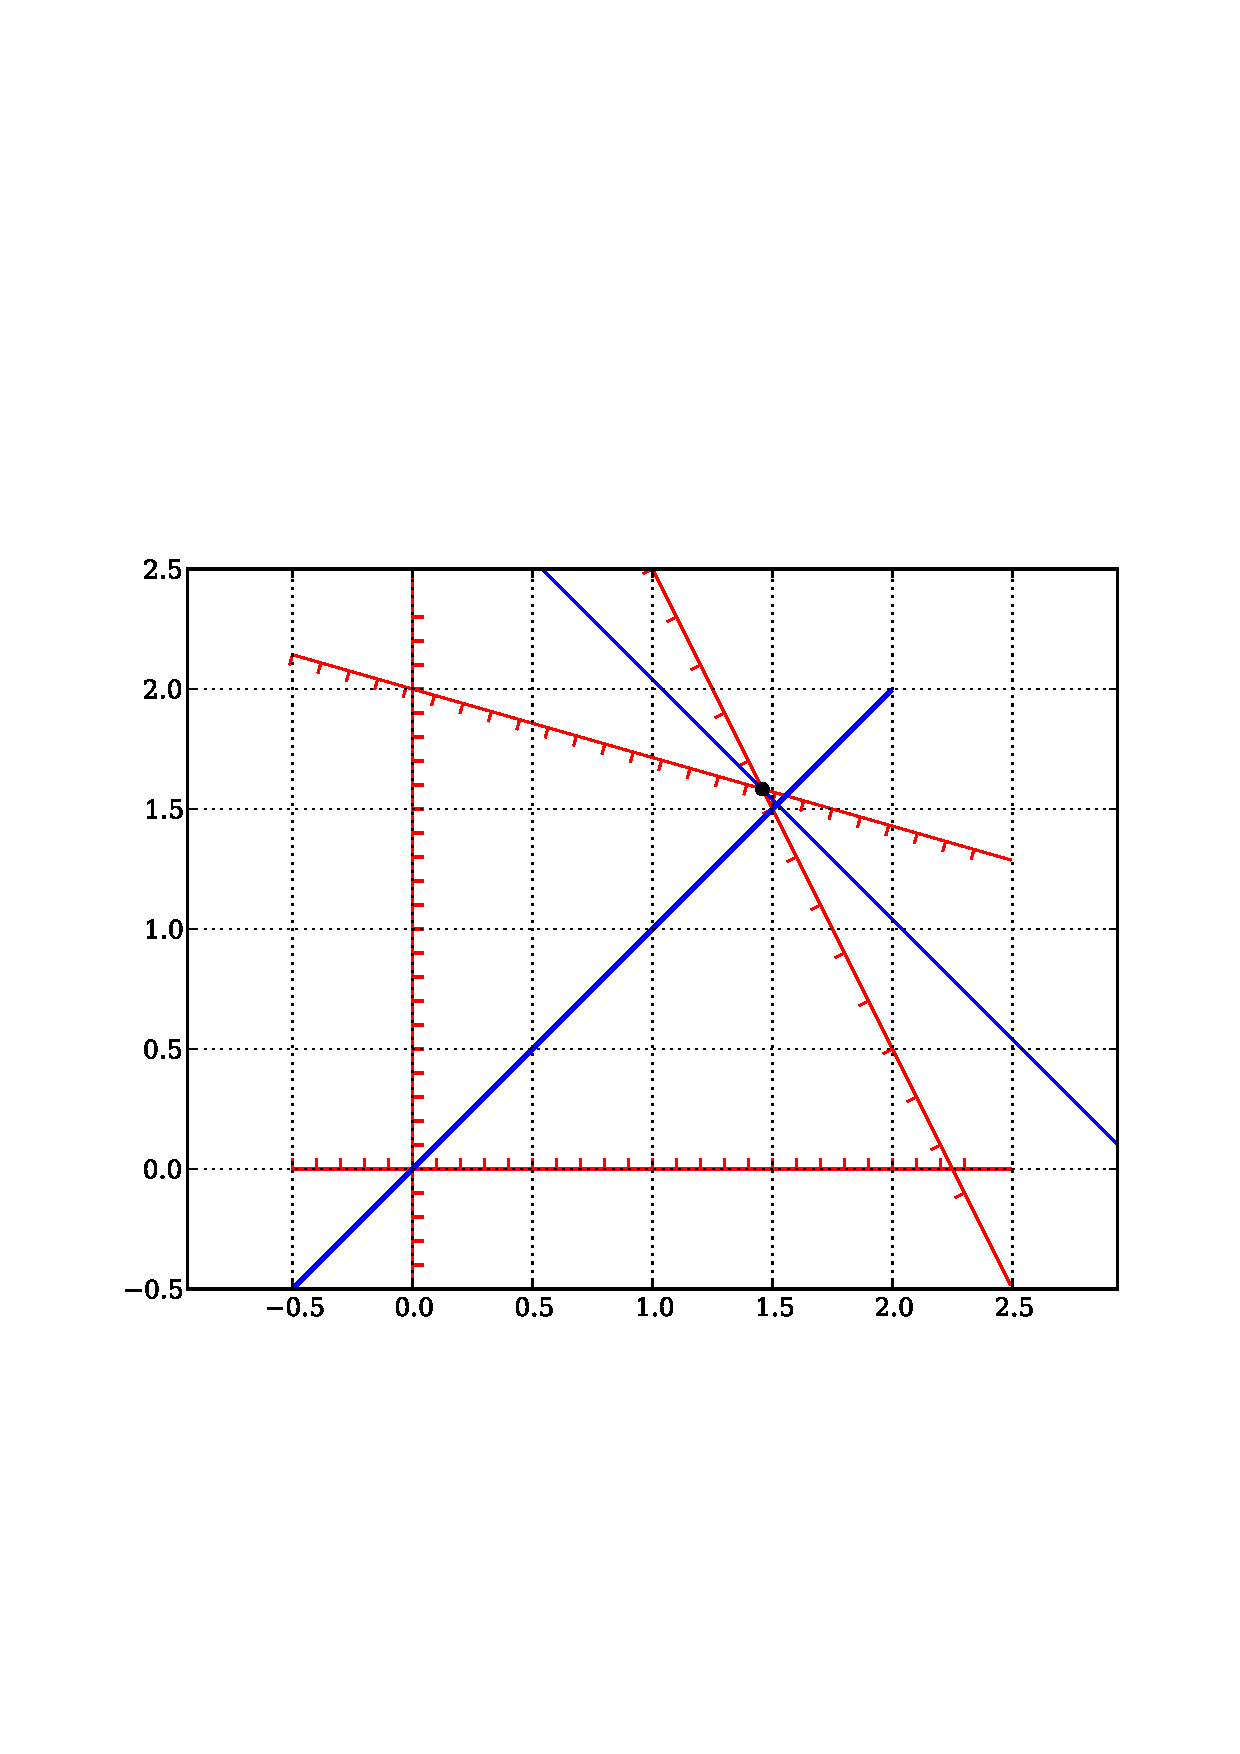
\includegraphics[width=\textwidth]{img/11}
\caption{Решение исходной ЗЛП графическим методом}
\end{figure}

\subsection{Решение двойственной ЗЛП}
Построим двойственную симметричную ЗЛП:

\begin{equation}
	Z(\vec{Y}) = 45 y_1 + 14y_2 \to min,
\end{equation}

\begin{equation}
\begin{cases}
20y_1 + 2y_2 \ge 1, \\
10y_1 + 7y_2 \ge 1, \\
y_1, y_2 \ge 0. \\
\end{cases}
\end{equation}

Введем искусственные переменные и приведем к каноническому виду.
\begin{equation}
	Z(\vec{Y}) = 45y_1+14y_2+Wy_5+Wy_6 \to min
\end{equation}

\begin{equation}
\begin{cases}
20y_1+2y_2-y_3+ s_5=1\\
10y_1+7y_2-y_4+ s_6=1\\
y_i, s_i \ge 0 \\
\end{cases}
\end{equation}
\begin{center}
\begin{tabular*}{\textwidth}{@{\extracolsep{\fill}}|c|c|c|c|c|c|c|c|c|c|c|}
\hline
$i$ & Базис & $B_i$ & C & $B_1 = 45$ & $B_2 = 14$ & $B_3 = 0$ & $B_4 = 0$ & $B_5 = W$ & $B_6 = W$ & $\Theta_i$ \\
\hline
$1$ & $P_5$ & W & $1$ & $20$ & $2$ & $-1$ & $0$ & $1$ & $0$ & $0,05$\\
$2$ & $P_6$ & W & $1$ & $10$ & $7$ & $0$ & $-1$ & $0$ & $1$ & $0,1$\\
\hline
$m+1$ & ~ & ~ & $0$ & $-45$ & $-14$ & $0$ & $0$ & $0$ & $0$ & ~ \\
\hline
$m+2$ & ~ & ~ & $2W$ & $30W$ & $9W$ & $-1W$ & $-1W$ & $0W$ & $0W$ & ~ \\
\hline
\end{tabular*}
\end{center}
\begin{center}
\begin{tabular*}{\textwidth}{@{\extracolsep{\fill}}|c|c|c|c|c|c|c|c|c|c|c|}
\hline
$i$ & Базис & $B_i$ & C & $B_1 = 45$ & $B_2 = 14$ & $B_3 = 0$ & $B_4 = 0$ & $B_5 = W$ & $B_6 = W$ & $\Theta_i$ \\
\hline
$1$ & $P_1$ & $45$ & $0,05$ & $1$ & $0,1$ & $-0,05$ & $0$ & $0,05$ & $0$ & $0,5$\\
$2$ & $P_6$ & W & $0,5$ & $0$ & $6$ & $0,5$ & $-1$ & $-0,5$ & $1$ & $0,08333$\\
\hline
$m+1$ & ~ & ~ & $2,25$ & $0$ & $-9,5$ & $-2,25$ & $0$ & $2,25$ & $0$ & ~ \\
\hline
$m+2$ & ~ & ~ & $0,5W$ & $0W$ & $6W$ & $0,5W$ & $-1W$ & $-1,5W$ & $0W$ & ~ \\
\hline
\end{tabular*}
\end{center}
\begin{center}
\begin{tabular*}{\textwidth}{@{\extracolsep{\fill}}|c|c|c|c|c|c|c|c|c|c|c|}
\hline
$i$ & Базис & $B_i$ & C & $B_1 = 45$ & $B_2 = 14$ & $B_3 = 0$ & $B_4 = 0$ & $B_5 = W$ & $B_6 = W$ & $\Theta_i$ \\
\hline
$1$ & $P_1$ & $45$ & $0,04167$ & $1$ & $0$ & $-0,05833$ & $0,01667$ & $0,05833$ & $-0,01667$ & ~\\
$2$ & $P_2$ & $14$ & $0,08333$ & $0$ & $1$ & $0,08333$ & $-0,1667$ & $-0,08333$ & $0,1667$ & ~\\
\hline
~ & ~ & ~ & $3,042$ & $0$ & $0$ & $-1,458$ & $-1,583$ & $1,458$ & $1,583$ & ~ \\
\hline
~ & ~ & ~ & $0W$ & $0W$ & $0W$ & $0W$ & $0W$ & $-1W$ & $-1W$ & ~ \\
\hline
\end{tabular*}
\end{center}
Получен оптимальный план: $Y^{опт} = (0,0417;0,0833)$, и оптимальное значение целевой функции $Z^{опт} = 3,04$.
\clearpage
\begin{figure}[ht]
\centering
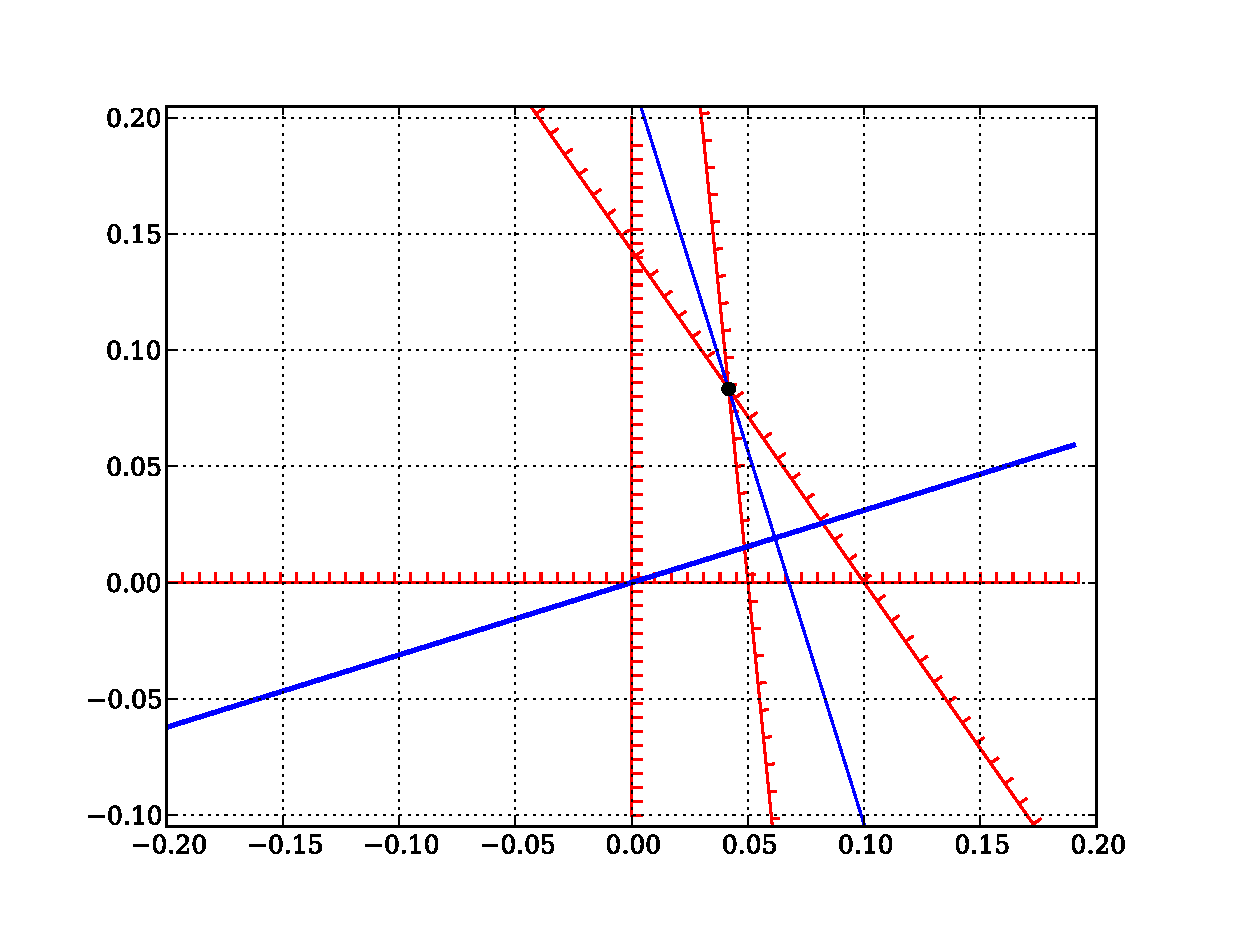
\includegraphics[width=0.9\textwidth]{img/12}
\caption{Решение двойственной задачи графическим методом}
\end{figure}

\subsection{Решение исходной и двойственное ЗЛП в программе}
Введем исходную и двойственную ЗЛП в программу и сравним результаты.

\begin{figure}[hb]
\centering
\includegraphics[scale=1.0]{img/problem11.png}
\caption{Условие задачи в программе}
\end{figure}
\newpage
\clearpage

\begin{figure}[ht]
\centering
\includegraphics[scale=1.0]{img/solution11.png}
\caption{Решение задачи в программе}
\end{figure}

\begin{figure}[ht]
\centering
\includegraphics[scale=1.0]{img/problem12.png}
\caption{Условие двойственной задачи в программе}
\end{figure}

\begin{figure}[ht]
\centering
\includegraphics[scale=1.0]{img/solution12.png}
\caption{Решение двойственной задачи в программе}
\end{figure}

\clearpage

\section{Пример II}

\subsection{Постановка задачи}
\renewcommand{\labelenumi}{\arabic{enumi})}
Задана ЗЛП в каноническом виде:
\begin{equation}
	F(\vec{X}) = 2x_1 - 5x_2 - x_3 + x_4 \to max,
\end{equation}

\begin{equation}
\begin{cases}
x_1 + 3x_2 - x_3 + x_4 = 1 \\
2x_1 + 3x_3 - x_4 = 2 \\
x_1, x_2, x_3, x_4 \ge 0
\end{cases}
\end{equation}.

Необходимо:
\begin{enumerate}
\item Решить исходную ЗЛП методом искусственного базиса;
\item Решить исходную ЗЛП графически;
\end{enumerate}

\subsection{Решение исходной ЗЛП методом искусственного базиса}
Введем искусственные переменные и приведем к каноническому виду.
Для нахождения максимума, умножим целевую функцию на -1.
Заметим, что вектор во втором столбце уже является
единичным после деления строки на 3.

$$-F(\vec{X}) = -(-2x_1+5x_2+x_3-x_4+Wx_5) \to max$$
\begin{equation}
\label{cannonical}
\begin{cases}
\frac{1}{3} x_1+x_2 - \frac{1}{3} x_3 + \frac{1}{3} x_4=\frac{1}{3} \\
2x_1+3x_3-x_4+ s_5=2\\
x_i, s_i \ge 0 \\
\end{cases}
\end{equation}

\begin{center}
\begin{tabular*}{\textwidth}{@{\extracolsep{\fill}}|c|c|c|c|c|c|c|c|c|c|}
\hline
$i$ & Базис & $C_i$ & B & $C_1 = -2$ & $C_2 = 5$ & $C_3 = 1$ & $C_4 = -1$ & $C_5 = W$ & $\Theta_i$ \\
\hline
$1$ & $P_2$ & $5$ & $0,3333$ & $0,3333$ & $1$ & $-0,3333$ & $0,3333$ & $0$ & --\\
$2$ & $P_5$ & W & $2$ & $2$ & $0$ & $3$ & $-1$ & $1$ & $0,6667$\\
\hline
$m+1$ & ~ & ~ & $1,667$ & $3,667$ & $0$ & $-2,667$ & $2,667$ & $0$ & ~ \\
\hline
$m+2$ & ~ & ~ & $2W$ & $2W$ & $0W$ & $3W$ & $-1W$ & $0W$ & ~ \\
\hline
\end{tabular*}
\end{center}
\begin{center}
\begin{tabular*}{\textwidth}{@{\extracolsep{\fill}}|c|c|c|c|c|c|c|c|c|c|}
\hline
$i$ & Базис & $C_i$ & B & $C_1 = -2$ & $C_2 = 5$ & $C_3 = 1$ & $C_4 = -1$ & $C_5 = W$ & $\Theta_i$ \\
\hline
$1$ & $P_2$ & $5$ & $0,5556$ & $0,5556$ & $1$ & $0$ & $0,2222$ & $0,1111$ & $1$\\
$2$ & $P_3$ & $1$ & $0,6667$ & $0,6667$ & $0$ & $1$ & $-0,3333$ & $0,3333$ & $1$\\
\hline
$m+1$ & ~ & ~ & $3,444$ & $5,444$ & $0$ & $0$ & $1,778$ & $0,8889$ & ~ \\
\hline
$m+2$ & ~ & ~ & $0W$ & $0W$ & $0W$ & $0W$ & $0W$ & $-1W$ & ~ \\
\hline
\end{tabular*}
\end{center}
\begin{center}
\begin{tabular*}{\textwidth}{@{\extracolsep{\fill}}|c|c|c|c|c|c|c|c|c|c|}
\hline
$i$ & Базис & $C_i$ & B & $C_1 = -2$ & $C_2 = 5$ & $C_3 = 1$ & $C_4 = -1$ & $C_5 = W$ & $\Theta_i$ \\
\hline
$1$ & $P_1$ & $-2$ & $1$ & $1$ & $1,8$ & $0$ & $0,4$ & $0,2$ & $1$\\
$2$ & $P_3$ & $1$ & $0$ & $0$ & $-1,2$ & $1$ & $-0,6$ & $0,2$ & $1$\\
\hline
$m+1$ & ~ & ~ & $-2$ & $0$ & $-9,8$ & $0$ & $-0,4$ & $-0,2$ & ~ \\
\hline
$m+2$ & ~ & ~ & $0W$ & $0W$ & $0W$ & $0W$ & $0W$ & $-1W$ & ~ \\
\hline
\end{tabular*}
\end{center}
Получен оптимальный план: $X^{опт} = (1;0;0;0;0)$,
и оптимальное значение целевой функции $F^{опт} = 2$.

\subsection{Решение исходной ЗЛП графическим методом}
\begin{figure}[ht]
\centering
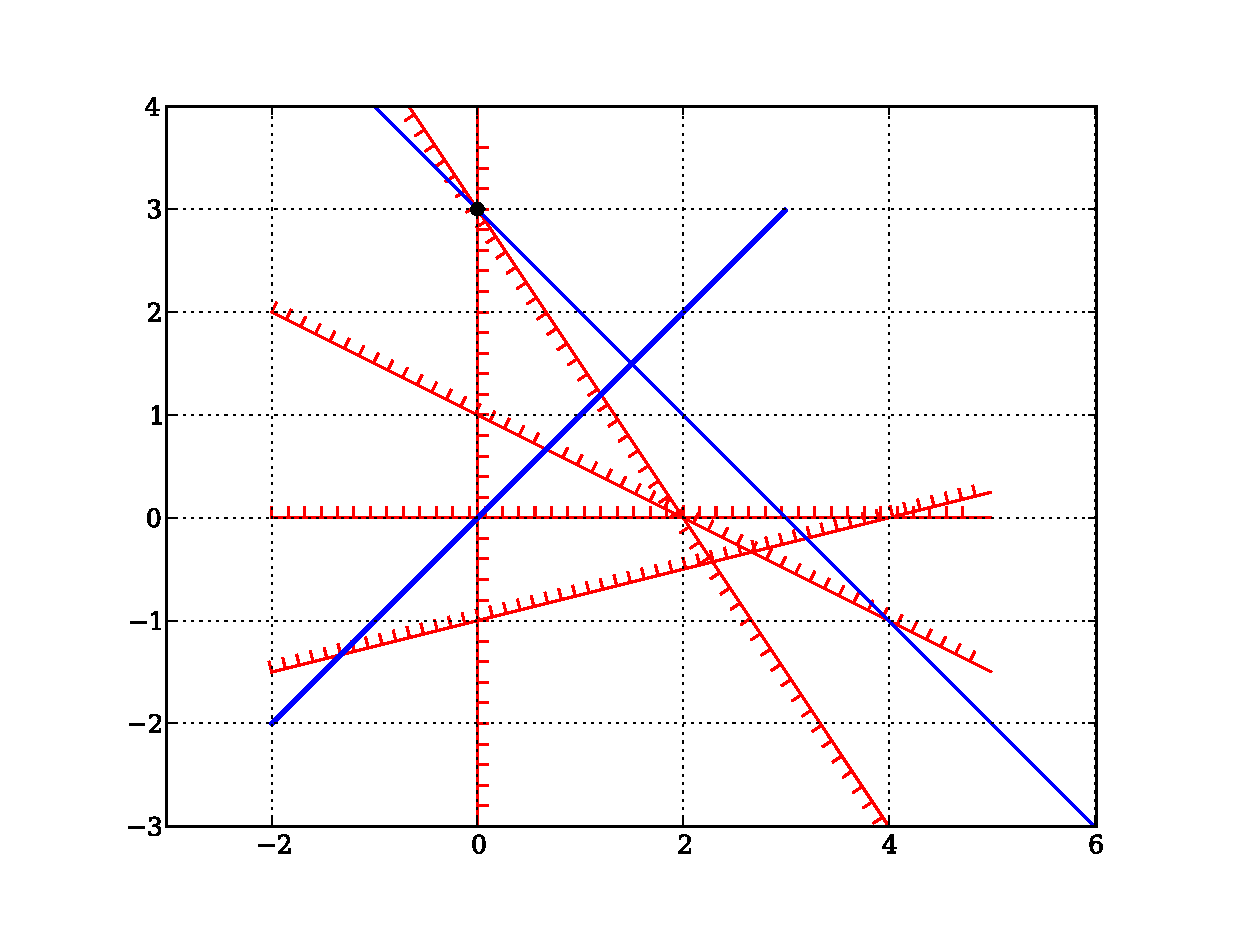
\includegraphics[width=\textwidth]{img/21}
\caption{Решение графическим методом}\label{21}
\end{figure}
\section{Пример III}
Задана ЗЛП:
$$F(\vec{X}) = x_1+4x_2 \to max$$
\begin{equation}
\label{system}
\begin{cases}
2x_1+4x_2 \le 17\\
10x_1+3x_2 \le 15\\
x_i \ge 0 \\
\end{cases}
\end{equation}

\subsection{Решение исходной ЗЛП}
Введем искусственные переменные и приведем к каноническому виду.
Для нахождения максимума, умножим целевую функцию на -1.

$$-F(\vec{X}) = -(-x_1-4x_2) \to max$$
\begin{equation}
\label{cannonical}
\begin{cases}
2x_1+4x_2+x_3=17\\
10x_1+3x_2+x_4=15\\
x_i, s_i \ge 0 \\
\end{cases}
\end{equation}

\begin{center}
\begin{tabular*}{\textwidth}{@{\extracolsep{\fill}}|c|c|c|c|c|c|c|c|c|}
\hline
$i$ & Базис & $C_i$ & B & $C_1 = -1$ & $C_2 = -4$ & $C_3 = 0$ & $C_4 = 0$ & $\Theta_i$ \\
\hline
$1$ & $P_3$ & $0$ & $17$ & $2$ & $4$ & $1$ & $0$ & $4,25$\\
$2$ & $P_4$ & $0$ & $15$ & $10$ & $3$ & $0$ & $1$ & $5$\\
\hline
$m+1$ & ~ & ~ & $0$ & $1$ & $4$ & $0$ & $0$ & ~ \\
\hline
\end{tabular*}
\end{center}
\begin{center}
\begin{tabular*}{\textwidth}{@{\extracolsep{\fill}}|c|c|c|c|c|c|c|c|c|}
\hline
$i$ & Базис & $C_i$ & B & $C_1 = -1$ & $C_2 = -4$ & $C_3 = 0$ & $C_4 = 0$ & $\Theta_i$ \\
\hline
$1$ & $P_2$ & $-4$ & $4,25$ & $0,5$ & $1$ & $0,25$ & $0$ & $4,25$\\
$2$ & $P_4$ & $0$ & $2,25$ & $8,5$ & $0$ & $-0,75$ & $1$ & $5$\\
\hline
$m+1$ & ~ & ~ & $-17$ & $0$ & $0$ & $-1$ & $0$ & ~ \\
\hline
\end{tabular*}
\end{center}
Получен оптимальный план: $X^{опт} = (0;4,25)$, и оптимальное значение целевой функции $F^{опт} = 17$.

\subsection{Нахождение целочисленных решений}
Компонент $P_2$ полученного плана не является целочисленным. Применим алгоритм Гомори.
Первое отсечение:
\begin{equation}
-0,5 x_1 - 0,25 x_3 + U_1 = -0,25.
\end{equation}
\begin{center}
\begin{tabular*}{\textwidth}{@{\extracolsep{\fill}}|c|c|c|c|c|c|c|c|c|c|}
\hline
$i$ & Базис & $C_i$ & B & $C_1 = -1$ & $C_2 = -4$ & $C_3 = 0$ & $C_4 = 0$ & $C_5 = 0$ & $\Theta_i$ \\
\hline
$1$ & $P_2$ & $-4$ & $4,25$ & $0,5$ & $1$ & $0,25$ & $0$ & $0$ & --\\
$2$ & $P_4$ & $0$ & $2,25$ & $8,5$ & $0$ & $-0,75$ & $1$ & $0$ & --\\
$3$ & $P_5$ & $0$ & $-0,25$ & $-0,5$ & $0$ & $-0,25$ & $0$ & $1$ & --\\
\hline
$m+1$ & ~ & ~ & $-17$ & $0$ & $0$ & $0$ & $0$ & $0$ & ~ \\
\hline
\end{tabular*}
\end{center}
\begin{center}
\begin{tabular*}{\textwidth}{@{\extracolsep{\fill}}|c|c|c|c|c|c|c|c|c|c|}
\hline
$i$ & Базис & $C_i$ & B & $C_1 = -1$ & $C_2 = -4$ & $C_3 = 0$ & $C_4 = 0$ & $C_5 = 0$ & $\Theta_i$ \\
\hline
$1$ & $P_2$ & $-4$ & $4$ & $0$ & $1$ & $0$ & $0$ & $1$ & --\\
$2$ & $P_4$ & $0$ & $-2$ & $0$ & $0$ & $-5$ & $1$ & $17$ & --\\
$3$ & $P_1$ & $-1$ & $0,5$ & $1$ & $0$ & $0,5$ & $0$ & $-2$ & --\\
\hline
$m+1$ & ~ & ~ & $-17$ & $0$ & $0$ & $0$ & $0$ & $0$ & ~ \\
\hline
\end{tabular*}
\end{center}
Второе отсечение:
\begin{equation}
- 0,5 x_3  + U_2 = -0,5.
\end{equation}
\begin{center}
\begin{tabular*}{\textwidth}{@{\extracolsep{\fill}}|c|c|c|c|c|c|c|c|c|c|c|}
\hline
$i$ & Базис & $C_i$ & B & $C_1 = -1$ & $C_2 = -4$ & $C_3 = 0$ & $C_4 = 0$ & $C_5 = 0$ & $C_6 = 0$ & $\Theta_i$ \\
\hline
$1$ & $P_2$ & $-4$ & $4$ & $0$ & $1$ & $0$ & $0$ & $1$ & $0$ & --\\
$2$ & $P_4$ & $0$ & $-2$ & $0$ & $0$ & $-5$ & $1$ & $17$ & $0$ & --\\
$3$ & $P_1$ & $-1$ & $0,5$ & $1$ & $0$ & $0,5$ & $0$ & $-2$ & $0$ & --\\
$4$ & $P_6$ & $0$ & $-0,5$ & $0$ & $0$ & $-0,5$ & $0$ & $0$ & $1$ & --\\
\hline
$m+1$ & ~ & ~ & $-17$ & $0$ & $0$ & $0$ & $0$ & $0$ & $0$ & ~ \\
\hline
\end{tabular*}
\end{center}
\begin{center}
\begin{tabular*}{\textwidth}{@{\extracolsep{\fill}}|c|c|c|c|c|c|c|c|c|c|c|}
\hline
$i$ & Базис & $C_i$ & B & $C_1 = -1$ & $C_2 = -4$ & $C_3 = 0$ & $C_4 = 0$ & $C_5 = 0$ & $C_6 = 0$ & $\Theta_i$ \\
\hline
$1$ & $P_2$ & $-4$ & $4$ & $0$ & $1$ & $0$ & $0$ & $1$ & $0$ & --\\
$2$ & $P_4$ & $0$ & $3$ & $0$ & $0$ & $0$ & $1$ & $17$ & $-10$ & --\\
$3$ & $P_1$ & $-1$ & $0$ & $1$ & $0$ & $0$ & $0$ & $-2$ & $1$ & --\\
$4$ & $P_3$ & $0$ & $1$ & $0$ & $0$ & $1$ & $0$ & $0$ & $-2$ & --\\
\hline
$m+1$ & ~ & ~ & $-17$ & $0$ & $0$ & $0$ & $0$ & $0$ & $0$ & ~ \\
\hline
\end{tabular*}
\end{center}
Получен оптимальный план: $X^{опт} = (0;4)$, и оптимальное значение целевой функции $F^{опт} = 16$.

\newpage
\subsection{Решение ЗЛП в программе}
Введем ЗЛП в программу и сравним результаты.

\begin{figure}[hb]
\centering
\includegraphics[scale=1.0]{img/problem31.png}
\caption{Условие задачи в программе}
\end{figure}

\begin{figure}[ht]
\centering
\includegraphics[scale=1.0]{img/solution31.png}
\caption{Решение задачи в программе}
\end{figure}


\backmatter

\end{document}
